\documentclass[1p]{elsarticle_modified}
%\bibliographystyle{elsarticle-num}

%\usepackage[colorlinks]{hyperref}
%\usepackage{abbrmath_seonhwa} %\Abb, \Ascr, \Acal ,\Abf, \Afrak
\usepackage{amsfonts}
\usepackage{amssymb}
\usepackage{amsmath}
\usepackage{amsthm}
\usepackage{scalefnt}
\usepackage{amsbsy}
\usepackage{kotex}
\usepackage{caption}
\usepackage{subfig}
\usepackage{color}
\usepackage{graphicx}
\usepackage{xcolor} %% white, black, red, green, blue, cyan, magenta, yellow
\usepackage{float}
\usepackage{setspace}
\usepackage{hyperref}

\usepackage{tikz}
\usetikzlibrary{arrows}

\usepackage{multirow}
\usepackage{array} % fixed length table
\usepackage{hhline}

%%%%%%%%%%%%%%%%%%%%%
\makeatletter
\renewcommand*\env@matrix[1][\arraystretch]{%
	\edef\arraystretch{#1}%
	\hskip -\arraycolsep
	\let\@ifnextchar\new@ifnextchar
	\array{*\c@MaxMatrixCols c}}
\makeatother %https://tex.stackexchange.com/questions/14071/how-can-i-increase-the-line-spacing-in-a-matrix
%%%%%%%%%%%%%%%

\usepackage[normalem]{ulem}

\newcommand{\msout}[1]{\ifmmode\text{\sout{\ensuremath{#1}}}\else\sout{#1}\fi}
%SOURCE: \msout is \stkout macro in https://tex.stackexchange.com/questions/20609/strikeout-in-math-mode

\newcommand{\cancel}[1]{
	\ifmmode
	{\color{red}\msout{#1}}
	\else
	{\color{red}\sout{#1}}
	\fi
}

\newcommand{\add}[1]{
	{\color{blue}\uwave{#1}}
}

\newcommand{\replace}[2]{
	\ifmmode
	{\color{red}\msout{#1}}{\color{blue}\uwave{#2}}
	\else
	{\color{red}\sout{#1}}{\color{blue}\uwave{#2}}
	\fi
}

\newcommand{\Sol}{\mathcal{S}} %segment
\newcommand{\D}{D} %diagram
\newcommand{\A}{\mathcal{A}} %arc


%%%%%%%%%%%%%%%%%%%%%%%%%%%%%5 test

\def\sl{\operatorname{\textup{SL}}(2,\Cbb)}
\def\psl{\operatorname{\textup{PSL}}(2,\Cbb)}
\def\quan{\mkern 1mu \triangleright \mkern 1mu}

\theoremstyle{definition}
\newtheorem{thm}{Theorem}[section]
\newtheorem{prop}[thm]{Proposition}
\newtheorem{lem}[thm]{Lemma}
\newtheorem{ques}[thm]{Question}
\newtheorem{cor}[thm]{Corollary}
\newtheorem{defn}[thm]{Definition}
\newtheorem{exam}[thm]{Example}
\newtheorem{rmk}[thm]{Remark}
\newtheorem{alg}[thm]{Algorithm}

\newcommand{\I}{\sqrt{-1}}
\begin{document}

%\begin{frontmatter}
%
%\title{Boundary parabolic representations of knots up to 8 crossings}
%
%%% Group authors per affiliation:
%\author{Yunhi Cho} 
%\address{Department of Mathematics, University of Seoul, Seoul, Korea}
%\ead{yhcho@uos.ac.kr}
%
%
%\author{Seonhwa Kim} %\fnref{s_kim}}
%\address{Center for Geometry and Physics, Institute for Basic Science, Pohang, 37673, Korea}
%\ead{ryeona17@ibs.re.kr}
%
%\author{Hyuk Kim}
%\address{Department of Mathematical Sciences, Seoul National University, Seoul 08826, Korea}
%\ead{hyukkim@snu.ac.kr}
%
%\author{Seokbeom Yoon}
%\address{Department of Mathematical Sciences, Seoul National University, Seoul, 08826,  Korea}
%\ead{sbyoon15@snu.ac.kr}
%
%\begin{abstract}
%We find all boundary parabolic representation of knots up to 8 crossings.
%
%\end{abstract}
%\begin{keyword}
%    \MSC[2010] 57M25 
%\end{keyword}
%
%\end{frontmatter}

%\linenumbers
%\tableofcontents
%
\newcommand\colored[1]{\textcolor{white}{\rule[-0.35ex]{0.8em}{1.4ex}}\kern-0.8em\color{red} #1}%
%\newcommand\colored[1]{\textcolor{white}{ #1}\kern-2.17ex	\textcolor{white}{ #1}\kern-1.81ex	\textcolor{white}{ #1}\kern-2.15ex\color{red}#1	}

{\Large $\underline{12a_{0959}~(K12a_{0959})}$}

\setlength{\tabcolsep}{10pt}
\renewcommand{\arraystretch}{1.6}
\vspace{1cm}\begin{tabular}{m{100pt}>{\centering\arraybackslash}m{274pt}}
\multirow{5}{120pt}{
	\centering
	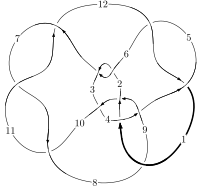
\includegraphics[width=112pt]{../../../GIT/diagram.site/Diagrams/png/1760_12a_0959.png}\\
\ \ \ A knot diagram\footnotemark}&
\allowdisplaybreaks
\textbf{Linearized knot diagam} \\
\cline{2-2}
 &
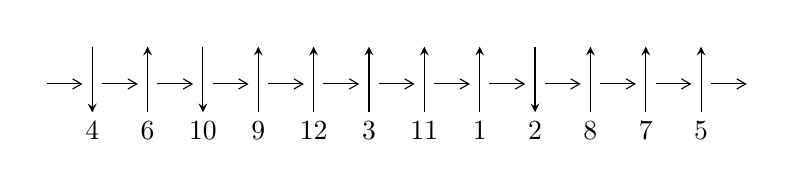
\begin{tikzpicture}[x=20pt, y=17pt]
	% nodes
	\node (C0) at (0, 0) {};
	\node (C1) at (1, 0) {};
	\node (C1U) at (1, +1) {};
	\node (C1D) at (1, -1) {4};

	\node (C2) at (2, 0) {};
	\node (C2U) at (2, +1) {};
	\node (C2D) at (2, -1) {6};

	\node (C3) at (3, 0) {};
	\node (C3U) at (3, +1) {};
	\node (C3D) at (3, -1) {10};

	\node (C4) at (4, 0) {};
	\node (C4U) at (4, +1) {};
	\node (C4D) at (4, -1) {9};

	\node (C5) at (5, 0) {};
	\node (C5U) at (5, +1) {};
	\node (C5D) at (5, -1) {12};

	\node (C6) at (6, 0) {};
	\node (C6U) at (6, +1) {};
	\node (C6D) at (6, -1) {3};

	\node (C7) at (7, 0) {};
	\node (C7U) at (7, +1) {};
	\node (C7D) at (7, -1) {11};

	\node (C8) at (8, 0) {};
	\node (C8U) at (8, +1) {};
	\node (C8D) at (8, -1) {1};

	\node (C9) at (9, 0) {};
	\node (C9U) at (9, +1) {};
	\node (C9D) at (9, -1) {2};

	\node (C10) at (10, 0) {};
	\node (C10U) at (10, +1) {};
	\node (C10D) at (10, -1) {8};

	\node (C11) at (11, 0) {};
	\node (C11U) at (11, +1) {};
	\node (C11D) at (11, -1) {7};

	\node (C12) at (12, 0) {};
	\node (C12U) at (12, +1) {};
	\node (C12D) at (12, -1) {5};
	\node (C13) at (13, 0) {};

	% arrows
	\draw[->,>={angle 60}]
	(C0) edge (C1) (C1) edge (C2) (C2) edge (C3) (C3) edge (C4) (C4) edge (C5) (C5) edge (C6) (C6) edge (C7) (C7) edge (C8) (C8) edge (C9) (C9) edge (C10) (C10) edge (C11) (C11) edge (C12) (C12) edge (C13) ;	\draw[->,>=stealth]
	(C1U) edge (C1D) (C2D) edge (C2U) (C3U) edge (C3D) (C4D) edge (C4U) (C5D) edge (C5U) (C6D) edge (C6U) (C7D) edge (C7U) (C8D) edge (C8U) (C9U) edge (C9D) (C10D) edge (C10U) (C11D) edge (C11U) (C12D) edge (C12U) ;
	\end{tikzpicture} \\
\hhline{~~} \\& 
\textbf{Solving Sequence} \\ \cline{2-2} 
 &
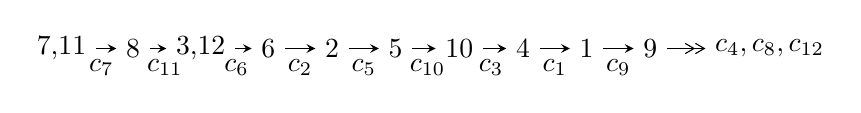
\begin{tikzpicture}[x=23pt, y=7pt]
	% node
	\node (A0) at (-1/8, 0) {7,11};
	\node (A1) at (1, 0) {8};
	\node (A2) at (33/16, 0) {3,12};
	\node (A3) at (25/8, 0) {6};
	\node (A4) at (33/8, 0) {2};
	\node (A5) at (41/8, 0) {5};
	\node (A6) at (49/8, 0) {10};
	\node (A7) at (57/8, 0) {4};
	\node (A8) at (65/8, 0) {1};
	\node (A9) at (73/8, 0) {9};
	\node (C1) at (1/2, -1) {$c_{7}$};
	\node (C2) at (3/2, -1) {$c_{11}$};
	\node (C3) at (21/8, -1) {$c_{6}$};
	\node (C4) at (29/8, -1) {$c_{2}$};
	\node (C5) at (37/8, -1) {$c_{5}$};
	\node (C6) at (45/8, -1) {$c_{10}$};
	\node (C7) at (53/8, -1) {$c_{3}$};
	\node (C8) at (61/8, -1) {$c_{1}$};
	\node (C9) at (69/8, -1) {$c_{9}$};
	\node (A10) at (11, 0) {$c_{4},c_{8},c_{12}$};

	% edge
	\draw[->,>=stealth]	
	(A0) edge (A1) (A1) edge (A2) (A2) edge (A3) (A3) edge (A4) (A4) edge (A5) (A5) edge (A6) (A6) edge (A7) (A7) edge (A8) (A8) edge (A9) ;
	\draw[->>,>={angle 60}]	
	(A9) edge (A10);
\end{tikzpicture} \\ 

\end{tabular} \\

\footnotetext{
The image of knot diagram is generated by the software ``\textbf{Draw programme}" developed by Andrew Bartholomew(\url{http://www.layer8.co.uk/maths/draw/index.htm\#Running-draw}), where we modified some parts for our purpose(\url{https://github.com/CATsTAILs/LinksPainter}).
}\phantom \\ \newline 
\centering \textbf{Ideals for irreducible components\footnotemark of $X_{\text{par}}$} 
 
\begin{align*}
I^u_{1}&=\langle 
8.35200\times10^{510} u^{141}-4.09385\times10^{511} u^{140}+\cdots+2.45826\times10^{513} b-8.83000\times10^{512},\\
\phantom{I^u_{1}}&\phantom{= \langle  }6.00094\times10^{514} u^{141}-2.96953\times10^{515} u^{140}+\cdots+2.13869\times10^{515} a-1.26630\times10^{517},\\
\phantom{I^u_{1}}&\phantom{= \langle  }u^{142}-5 u^{141}+\cdots-332 u+29\rangle \\
I^u_{2}&=\langle 
75418015 u^{30}+613925564 u^{29}+\cdots+89877703 b-104428676,\\
\phantom{I^u_{2}}&\phantom{= \langle  }227579646 u^{30}+1595720565 u^{29}+\cdots+89877703 a+471832864,\;u^{31}+6 u^{30}+\cdots+27 u^2-1\rangle \\
I^u_{3}&=\langle 
b-1,\;3 a- u+1,\;u^2+u+1\rangle \\
I^u_{4}&=\langle 
b-1,\;a+u,\;u^2+u+1\rangle \\
\\
\end{align*}
\raggedright * 4 irreducible components of $\dim_{\mathbb{C}}=0$, with total 177 representations.\\
\footnotetext{All coefficients of polynomials are rational numbers. But the coefficients are sometimes approximated in decimal forms when there is not enough margin.}
\newpage
\renewcommand{\arraystretch}{1}
\centering \section*{I. $I^u_{1}= \langle 8.35\times10^{510} u^{141}-4.09\times10^{511} u^{140}+\cdots+2.46\times10^{513} b-8.83\times10^{512},\;6.00\times10^{514} u^{141}-2.97\times10^{515} u^{140}+\cdots+2.14\times10^{515} a-1.27\times10^{517},\;u^{142}-5 u^{141}+\cdots-332 u+29 \rangle$}
\flushleft \textbf{(i) Arc colorings}\\
\begin{tabular}{m{7pt} m{180pt} m{7pt} m{180pt} }
\flushright $a_{7}=$&$\begin{pmatrix}1\\0\end{pmatrix}$ \\
\flushright $a_{11}=$&$\begin{pmatrix}0\\u\end{pmatrix}$ \\
\flushright $a_{8}=$&$\begin{pmatrix}1\\- u^2\end{pmatrix}$ \\
\flushright $a_{3}=$&$\begin{pmatrix}-0.280590 u^{141}+1.38848 u^{140}+\cdots-228.267 u+59.2090\\-0.00339752 u^{141}+0.0166534 u^{140}+\cdots+1.73708 u+0.359197\end{pmatrix}$ \\
\flushright $a_{12}=$&$\begin{pmatrix}u\\u\end{pmatrix}$ \\
\flushright $a_{6}=$&$\begin{pmatrix}-0.161778 u^{141}+0.754742 u^{140}+\cdots-182.653 u+47.6645\\0.0494736 u^{141}-0.275149 u^{140}+\cdots+7.41354 u-0.302281\end{pmatrix}$ \\
\flushright $a_{2}=$&$\begin{pmatrix}0.000859398 u^{141}+0.0173947 u^{140}+\cdots-87.6362 u+22.3884\\0.0988280 u^{141}-0.484196 u^{140}+\cdots-0.641859 u+0.706963\end{pmatrix}$ \\
\flushright $a_{5}=$&$\begin{pmatrix}-0.174032 u^{141}+0.814178 u^{140}+\cdots-185.281 u+48.4292\\0.0372198 u^{141}-0.215713 u^{140}+\cdots+4.78579 u+0.462379\end{pmatrix}$ \\
\flushright $a_{10}=$&$\begin{pmatrix}- u\\u^3+u\end{pmatrix}$ \\
\flushright $a_{4}=$&$\begin{pmatrix}-0.267746 u^{141}+1.28141 u^{140}+\cdots-216.097 u+57.4617\\-0.00572144 u^{141}-0.00711253 u^{140}+\cdots+4.17014 u+0.863544\end{pmatrix}$ \\
\flushright $a_{1}=$&$\begin{pmatrix}0.400381 u^{141}-1.89645 u^{140}+\cdots+318.441 u-68.7080\\0.0321004 u^{141}-0.116898 u^{140}+\cdots-13.3500 u+3.03495\end{pmatrix}$ \\
\flushright $a_{9}=$&$\begin{pmatrix}0.228624 u^{141}-1.18663 u^{140}+\cdots+64.1107 u-11.5201\\0.199469 u^{141}-1.13061 u^{140}+\cdots+19.9646 u-0.792164\end{pmatrix}$\\&\end{tabular}
\flushleft \textbf{(ii) Obstruction class $= -1$}\\~\\
\flushleft \textbf{(iii) Cusp Shapes $= 2.49543 u^{141}-12.0492 u^{140}+\cdots+2253.52 u-500.102$}\\~\\
\newpage\renewcommand{\arraystretch}{1}
\flushleft \textbf{(iv) u-Polynomials at the component}\newline \\
\begin{tabular}{m{50pt}|m{274pt}}
Crossings & \hspace{64pt}u-Polynomials at each crossing \\
\hline $$\begin{aligned}c_{1}\end{aligned}$$&$\begin{aligned}
&3(3 u^{142}-20 u^{140}+\cdots+29 u-1)
\end{aligned}$\\
\hline $$\begin{aligned}c_{2},c_{6}\end{aligned}$$&$\begin{aligned}
&u^{142}+2 u^{141}+\cdots-356 u+304
\end{aligned}$\\
\hline $$\begin{aligned}c_{3}\end{aligned}$$&$\begin{aligned}
&3(3 u^{142}-6 u^{141}+\cdots-261246 u-14332)
\end{aligned}$\\
\hline $$\begin{aligned}c_{4}\end{aligned}$$&$\begin{aligned}
&u^{142}+2 u^{141}+\cdots+32895 u-13173
\end{aligned}$\\
\hline $$\begin{aligned}c_{5},c_{12}\end{aligned}$$&$\begin{aligned}
&3(3 u^{142}+12 u^{141}+\cdots-1.16737\times10^{7} u-729697)
\end{aligned}$\\
\hline $$\begin{aligned}c_{7},c_{10},c_{11}\end{aligned}$$&$\begin{aligned}
&u^{142}-5 u^{141}+\cdots-332 u+29
\end{aligned}$\\
\hline $$\begin{aligned}c_{8}\end{aligned}$$&$\begin{aligned}
&u^{142}+22 u^{140}+\cdots+3840 u+576
\end{aligned}$\\
\hline $$\begin{aligned}c_{9}\end{aligned}$$&$\begin{aligned}
&u^{142}-2 u^{141}+\cdots+29864 u-11279
\end{aligned}$\\
\hline
\end{tabular}\\~\\
\newpage\renewcommand{\arraystretch}{1}
\flushleft \textbf{(v) Riley Polynomials at the component}\newline \\
\begin{tabular}{m{50pt}|m{274pt}}
Crossings & \hspace{64pt}Riley Polynomials at each crossing \\
\hline $$\begin{aligned}c_{1}\end{aligned}$$&$\begin{aligned}
&9(9 y^{142}-120 y^{141}+\cdots-57 y+1)
\end{aligned}$\\
\hline $$\begin{aligned}c_{2},c_{6}\end{aligned}$$&$\begin{aligned}
&y^{142}-62 y^{141}+\cdots+425936 y+92416
\end{aligned}$\\
\hline $$\begin{aligned}c_{3}\end{aligned}$$&$\begin{aligned}
&9(9 y^{142}-138 y^{141}+\cdots+2.20180\times10^{10} y+2.05406\times10^{8})
\end{aligned}$\\
\hline $$\begin{aligned}c_{4}\end{aligned}$$&$\begin{aligned}
&y^{142}+26 y^{141}+\cdots+7659337353 y+173527929
\end{aligned}$\\
\hline $$\begin{aligned}c_{5},c_{12}\end{aligned}$$&$\begin{aligned}
&9(9 y^{142}+852 y^{141}+\cdots+1.69390\times10^{13} y+5.32458\times10^{11})
\end{aligned}$\\
\hline $$\begin{aligned}c_{7},c_{10},c_{11}\end{aligned}$$&$\begin{aligned}
&y^{142}+139 y^{141}+\cdots-94158 y+841
\end{aligned}$\\
\hline $$\begin{aligned}c_{8}\end{aligned}$$&$\begin{aligned}
&y^{142}+44 y^{141}+\cdots-2230272 y+331776
\end{aligned}$\\
\hline $$\begin{aligned}c_{9}\end{aligned}$$&$\begin{aligned}
&y^{142}+2 y^{141}+\cdots-7484772366 y+127215841
\end{aligned}$\\
\hline
\end{tabular}\\~\\
\newpage\flushleft \textbf{(vi) Complex Volumes and Cusp Shapes}
$$\begin{array}{c|c|c}  
\text{Solutions to }I^u_{1}& \I (\text{vol} + \sqrt{-1}CS) & \text{Cusp shape}\\
 \hline 
\begin{aligned}
u &= \phantom{-}0.642590 + 0.816128 I \\
a &= \phantom{-}0.017475 - 0.603353 I \\
b &= -1.090570 - 0.186235 I\end{aligned}
 & \phantom{-}2.74568 + 3.72052 I & \phantom{-0.000000 } 0 \\ \hline\begin{aligned}
u &= \phantom{-}0.642590 - 0.816128 I \\
a &= \phantom{-}0.017475 + 0.603353 I \\
b &= -1.090570 + 0.186235 I\end{aligned}
 & \phantom{-}2.74568 - 3.72052 I & \phantom{-0.000000 } 0 \\ \hline\begin{aligned}
u &= \phantom{-}0.943307 + 0.013606 I \\
a &= \phantom{-}0.523454 - 0.510396 I \\
b &= -0.918496 - 0.691900 I\end{aligned}
 & \phantom{-}0.70494 + 2.70160 I & \phantom{-0.000000 } 0 \\ \hline\begin{aligned}
u &= \phantom{-}0.943307 - 0.013606 I \\
a &= \phantom{-}0.523454 + 0.510396 I \\
b &= -0.918496 + 0.691900 I\end{aligned}
 & \phantom{-}0.70494 - 2.70160 I & \phantom{-0.000000 } 0 \\ \hline\begin{aligned}
u &= -0.966558 + 0.452108 I \\
a &= -0.535878 - 0.706338 I \\
b &= \phantom{-}1.158380 - 0.655861 I\end{aligned}
 & -1.3841 - 14.7096 I & \phantom{-0.000000 } 0 \\ \hline\begin{aligned}
u &= -0.966558 - 0.452108 I \\
a &= -0.535878 + 0.706338 I \\
b &= \phantom{-}1.158380 + 0.655861 I\end{aligned}
 & -1.3841 + 14.7096 I & \phantom{-0.000000 } 0 \\ \hline\begin{aligned}
u &= \phantom{-}0.875728 + 0.317953 I \\
a &= \phantom{-}0.439140 - 0.569516 I \\
b &= -1.044380 - 0.109811 I\end{aligned}
 & \phantom{-}4.26985 + 1.50980 I & \phantom{-0.000000 } 0 \\ \hline\begin{aligned}
u &= \phantom{-}0.875728 - 0.317953 I \\
a &= \phantom{-}0.439140 + 0.569516 I \\
b &= -1.044380 + 0.109811 I\end{aligned}
 & \phantom{-}4.26985 - 1.50980 I & \phantom{-0.000000 } 0 \\ \hline\begin{aligned}
u &= \phantom{-}0.493472 + 0.961325 I \\
a &= -0.340616 - 0.322389 I \\
b &= \phantom{-}1.089300 - 0.079315 I\end{aligned}
 & \phantom{-}1.53464 + 2.38535 I & \phantom{-0.000000 } 0 \\ \hline\begin{aligned}
u &= \phantom{-}0.493472 - 0.961325 I \\
a &= -0.340616 + 0.322389 I \\
b &= \phantom{-}1.089300 + 0.079315 I\end{aligned}
 & \phantom{-}1.53464 - 2.38535 I & \phantom{-0.000000 } 0\\
 \hline 
 \end{array}$$\newpage$$\begin{array}{c|c|c}  
\text{Solutions to }I^u_{1}& \I (\text{vol} + \sqrt{-1}CS) & \text{Cusp shape}\\
 \hline 
\begin{aligned}
u &= -0.790119 + 0.452760 I \\
a &= -1.356870 - 0.396797 I \\
b &= \phantom{-}0.728522 - 0.516306 I\end{aligned}
 & -3.29487 + 4.30574 I & \phantom{-0.000000 } 0 \\ \hline\begin{aligned}
u &= -0.790119 - 0.452760 I \\
a &= -1.356870 + 0.396797 I \\
b &= \phantom{-}0.728522 + 0.516306 I\end{aligned}
 & -3.29487 - 4.30574 I & \phantom{-0.000000 } 0 \\ \hline\begin{aligned}
u &= \phantom{-}0.208817 + 1.079900 I \\
a &= -0.223436 + 0.626423 I \\
b &= -0.429029 + 0.204141 I\end{aligned}
 & -2.34458 + 3.04452 I & \phantom{-0.000000 } 0 \\ \hline\begin{aligned}
u &= \phantom{-}0.208817 - 1.079900 I \\
a &= -0.223436 - 0.626423 I \\
b &= -0.429029 - 0.204141 I\end{aligned}
 & -2.34458 - 3.04452 I & \phantom{-0.000000 } 0 \\ \hline\begin{aligned}
u &= \phantom{-}1.020410 + 0.442473 I \\
a &= -0.521102 + 0.238186 I \\
b &= \phantom{-}1.088850 + 0.444342 I\end{aligned}
 & \phantom{-}0.64936 + 4.75757 I & \phantom{-0.000000 } 0 \\ \hline\begin{aligned}
u &= \phantom{-}1.020410 - 0.442473 I \\
a &= -0.521102 - 0.238186 I \\
b &= \phantom{-}1.088850 - 0.444342 I\end{aligned}
 & \phantom{-}0.64936 - 4.75757 I & \phantom{-0.000000 } 0 \\ \hline\begin{aligned}
u &= \phantom{-}0.707431 + 0.499654 I \\
a &= -0.386233 + 0.646196 I \\
b &= \phantom{-}1.219560 + 0.648628 I\end{aligned}
 & -1.03167 + 5.58242 I & \phantom{-0.000000 } 0 \\ \hline\begin{aligned}
u &= \phantom{-}0.707431 - 0.499654 I \\
a &= -0.386233 - 0.646196 I \\
b &= \phantom{-}1.219560 - 0.648628 I\end{aligned}
 & -1.03167 - 5.58242 I & \phantom{-0.000000 } 0 \\ \hline\begin{aligned}
u &= \phantom{-}0.749048 + 0.402762 I \\
a &= -0.087163 + 1.372770 I \\
b &= \phantom{-}0.981884 + 0.276958 I\end{aligned}
 & \phantom{-}3.02954 + 2.04599 I & \phantom{-0.000000 } 0 \\ \hline\begin{aligned}
u &= \phantom{-}0.749048 - 0.402762 I \\
a &= -0.087163 - 1.372770 I \\
b &= \phantom{-}0.981884 - 0.276958 I\end{aligned}
 & \phantom{-}3.02954 - 2.04599 I & \phantom{-0.000000 } 0\\
 \hline 
 \end{array}$$\newpage$$\begin{array}{c|c|c}  
\text{Solutions to }I^u_{1}& \I (\text{vol} + \sqrt{-1}CS) & \text{Cusp shape}\\
 \hline 
\begin{aligned}
u &= -0.737530 + 0.384331 I \\
a &= \phantom{-}0.857728 + 0.749010 I \\
b &= -1.154610 + 0.661050 I\end{aligned}
 & -2.52747 - 7.11688 I & \phantom{-0.000000 } 0 \\ \hline\begin{aligned}
u &= -0.737530 - 0.384331 I \\
a &= \phantom{-}0.857728 - 0.749010 I \\
b &= -1.154610 - 0.661050 I\end{aligned}
 & -2.52747 + 7.11688 I & \phantom{-0.000000 } 0 \\ \hline\begin{aligned}
u &= -0.643956 + 0.508889 I \\
a &= -0.338789 + 0.319747 I \\
b &= \phantom{-}0.376743 + 0.950292 I\end{aligned}
 & -3.72501 - 8.90092 I & \phantom{-0.000000 } 0 \\ \hline\begin{aligned}
u &= -0.643956 - 0.508889 I \\
a &= -0.338789 - 0.319747 I \\
b &= \phantom{-}0.376743 - 0.950292 I\end{aligned}
 & -3.72501 + 8.90092 I & \phantom{-0.000000 } 0 \\ \hline\begin{aligned}
u &= \phantom{-}1.065310 + 0.522095 I \\
a &= \phantom{-}0.583609 - 0.675353 I \\
b &= -0.995320 - 0.551462 I\end{aligned}
 & \phantom{-}0.87974 + 5.44723 I & \phantom{-0.000000 } 0 \\ \hline\begin{aligned}
u &= \phantom{-}1.065310 - 0.522095 I \\
a &= \phantom{-}0.583609 + 0.675353 I \\
b &= -0.995320 + 0.551462 I\end{aligned}
 & \phantom{-}0.87974 - 5.44723 I & \phantom{-0.000000 } 0 \\ \hline\begin{aligned}
u &= -0.693685 + 0.398764 I \\
a &= \phantom{-}0.451970 + 1.337320 I \\
b &= -1.211880 + 0.404517 I\end{aligned}
 & \phantom{-}3.98949 - 8.94716 I & \phantom{-0.000000 } 0 \\ \hline\begin{aligned}
u &= -0.693685 - 0.398764 I \\
a &= \phantom{-}0.451970 - 1.337320 I \\
b &= -1.211880 - 0.404517 I\end{aligned}
 & \phantom{-}3.98949 + 8.94716 I & \phantom{-0.000000 } 0 \\ \hline\begin{aligned}
u &= \phantom{-}0.340372 + 1.157210 I \\
a &= \phantom{-}0.34956 - 2.02425 I \\
b &= -0.821720 - 0.784733 I\end{aligned}
 & -2.82768 + 7.38570 I & \phantom{-0.000000 } 0 \\ \hline\begin{aligned}
u &= \phantom{-}0.340372 - 1.157210 I \\
a &= \phantom{-}0.34956 + 2.02425 I \\
b &= -0.821720 + 0.784733 I\end{aligned}
 & -2.82768 - 7.38570 I & \phantom{-0.000000 } 0\\
 \hline 
 \end{array}$$\newpage$$\begin{array}{c|c|c}  
\text{Solutions to }I^u_{1}& \I (\text{vol} + \sqrt{-1}CS) & \text{Cusp shape}\\
 \hline 
\begin{aligned}
u &= -0.333359 + 0.713404 I \\
a &= -0.475634 + 0.135045 I \\
b &= -1.303340 - 0.251159 I\end{aligned}
 & \phantom{-}3.04704 + 5.02224 I & \phantom{-0.000000 } 0 \\ \hline\begin{aligned}
u &= -0.333359 - 0.713404 I \\
a &= -0.475634 - 0.135045 I \\
b &= -1.303340 + 0.251159 I\end{aligned}
 & \phantom{-}3.04704 - 5.02224 I & \phantom{-0.000000 } 0 \\ \hline\begin{aligned}
u &= -0.240579 + 1.193860 I \\
a &= \phantom{-}0.932308 - 0.268323 I \\
b &= \phantom{-}1.380920 + 0.175400 I\end{aligned}
 & \phantom{-}0.47775 - 3.33774 I & \phantom{-0.000000 } 0 \\ \hline\begin{aligned}
u &= -0.240579 - 1.193860 I \\
a &= \phantom{-}0.932308 + 0.268323 I \\
b &= \phantom{-}1.380920 - 0.175400 I\end{aligned}
 & \phantom{-}0.47775 + 3.33774 I & \phantom{-0.000000 } 0 \\ \hline\begin{aligned}
u &= \phantom{-}0.548703 + 1.091500 I \\
a &= -0.527923 + 0.273988 I \\
b &= -0.823315 + 0.539077 I\end{aligned}
 & -2.62567 + 2.51585 I & \phantom{-0.000000 } 0 \\ \hline\begin{aligned}
u &= \phantom{-}0.548703 - 1.091500 I \\
a &= -0.527923 - 0.273988 I \\
b &= -0.823315 - 0.539077 I\end{aligned}
 & -2.62567 - 2.51585 I & \phantom{-0.000000 } 0 \\ \hline\begin{aligned}
u &= \phantom{-}0.853051 + 0.882884 I \\
a &= \phantom{-}0.186871 + 0.078567 I \\
b &= -0.689713 + 0.477853 I\end{aligned}
 & -0.187221 + 1.160760 I & \phantom{-0.000000 } 0 \\ \hline\begin{aligned}
u &= \phantom{-}0.853051 - 0.882884 I \\
a &= \phantom{-}0.186871 - 0.078567 I \\
b &= -0.689713 - 0.477853 I\end{aligned}
 & -0.187221 - 1.160760 I & \phantom{-0.000000 } 0 \\ \hline\begin{aligned}
u &= -0.163374 + 1.218340 I \\
a &= -1.02663 - 1.89218 I \\
b &= -0.092596 - 0.262769 I\end{aligned}
 & -4.71635 - 7.36833 I & \phantom{-0.000000 } 0 \\ \hline\begin{aligned}
u &= -0.163374 - 1.218340 I \\
a &= -1.02663 + 1.89218 I \\
b &= -0.092596 + 0.262769 I\end{aligned}
 & -4.71635 + 7.36833 I & \phantom{-0.000000 } 0\\
 \hline 
 \end{array}$$\newpage$$\begin{array}{c|c|c}  
\text{Solutions to }I^u_{1}& \I (\text{vol} + \sqrt{-1}CS) & \text{Cusp shape}\\
 \hline 
\begin{aligned}
u &= -0.871082 + 0.873688 I \\
a &= \phantom{-}0.224041 - 0.128263 I \\
b &= \phantom{-}0.956294 + 0.527645 I\end{aligned}
 & -2.54329 + 8.54907 I & \phantom{-0.000000 } 0 \\ \hline\begin{aligned}
u &= -0.871082 - 0.873688 I \\
a &= \phantom{-}0.224041 + 0.128263 I \\
b &= \phantom{-}0.956294 - 0.527645 I\end{aligned}
 & -2.54329 - 8.54907 I & \phantom{-0.000000 } 0 \\ \hline\begin{aligned}
u &= -0.509071 + 0.547445 I \\
a &= -0.157483 + 0.680723 I \\
b &= -0.867139 - 0.575732 I\end{aligned}
 & -3.33250 + 2.82467 I & \phantom{-0.000000 } 0 \\ \hline\begin{aligned}
u &= -0.509071 - 0.547445 I \\
a &= -0.157483 - 0.680723 I \\
b &= -0.867139 + 0.575732 I\end{aligned}
 & -3.33250 - 2.82467 I & \phantom{-0.000000 } 0 \\ \hline\begin{aligned}
u &= \phantom{-}0.328825 + 0.657498 I \\
a &= \phantom{-}0.704188 + 0.606675 I \\
b &= -0.008280 + 0.398492 I\end{aligned}
 & -0.40637 + 1.82781 I & \phantom{-0.000000 } 0 \\ \hline\begin{aligned}
u &= \phantom{-}0.328825 - 0.657498 I \\
a &= \phantom{-}0.704188 - 0.606675 I \\
b &= -0.008280 - 0.398492 I\end{aligned}
 & -0.40637 - 1.82781 I & \phantom{-0.000000 } 0 \\ \hline\begin{aligned}
u &= \phantom{-}0.097968 + 1.268690 I \\
a &= \phantom{-}0.78424 + 1.56513 I \\
b &= \phantom{-}0.746783 + 0.781991 I\end{aligned}
 & -1.52986 + 2.94544 I & \phantom{-0.000000 } 0 \\ \hline\begin{aligned}
u &= \phantom{-}0.097968 - 1.268690 I \\
a &= \phantom{-}0.78424 - 1.56513 I \\
b &= \phantom{-}0.746783 - 0.781991 I\end{aligned}
 & -1.52986 - 2.94544 I & \phantom{-0.000000 } 0 \\ \hline\begin{aligned}
u &= -0.006619 + 1.292480 I \\
a &= \phantom{-}0.13050 + 2.44173 I \\
b &= -0.133227 + 1.311720 I\end{aligned}
 & -7.54127 + 0.89803 I & \phantom{-0.000000 } 0 \\ \hline\begin{aligned}
u &= -0.006619 - 1.292480 I \\
a &= \phantom{-}0.13050 - 2.44173 I \\
b &= -0.133227 - 1.311720 I\end{aligned}
 & -7.54127 - 0.89803 I & \phantom{-0.000000 } 0\\
 \hline 
 \end{array}$$\newpage$$\begin{array}{c|c|c}  
\text{Solutions to }I^u_{1}& \I (\text{vol} + \sqrt{-1}CS) & \text{Cusp shape}\\
 \hline 
\begin{aligned}
u &= -0.168089 + 1.283240 I \\
a &= -0.94002 + 1.07137 I \\
b &= -0.964706 + 0.361388 I\end{aligned}
 & -1.70264 + 3.21989 I & \phantom{-0.000000 } 0 \\ \hline\begin{aligned}
u &= -0.168089 - 1.283240 I \\
a &= -0.94002 - 1.07137 I \\
b &= -0.964706 - 0.361388 I\end{aligned}
 & -1.70264 - 3.21989 I & \phantom{-0.000000 } 0 \\ \hline\begin{aligned}
u &= \phantom{-}0.057100 + 1.324370 I \\
a &= \phantom{-}0.345602 - 0.380089 I \\
b &= \phantom{-}1.49368 - 0.11239 I\end{aligned}
 & -1.23352 + 0.72597 I & \phantom{-0.000000 } 0 \\ \hline\begin{aligned}
u &= \phantom{-}0.057100 - 1.324370 I \\
a &= \phantom{-}0.345602 + 0.380089 I \\
b &= \phantom{-}1.49368 + 0.11239 I\end{aligned}
 & -1.23352 - 0.72597 I & \phantom{-0.000000 } 0 \\ \hline\begin{aligned}
u &= -0.201131 + 1.310480 I \\
a &= \phantom{-}0.39729 - 1.76605 I \\
b &= \phantom{-}1.119060 - 0.706966 I\end{aligned}
 & -0.30789 - 2.94943 I & \phantom{-0.000000 } 0 \\ \hline\begin{aligned}
u &= -0.201131 - 1.310480 I \\
a &= \phantom{-}0.39729 + 1.76605 I \\
b &= \phantom{-}1.119060 + 0.706966 I\end{aligned}
 & -0.30789 + 2.94943 I & \phantom{-0.000000 } 0 \\ \hline\begin{aligned}
u &= \phantom{-}0.558574 + 0.358142 I \\
a &= \phantom{-}0.31244 + 1.61475 I \\
b &= \phantom{-}0.941529 - 0.330493 I\end{aligned}
 & -0.83700 - 1.33766 I & \phantom{-0.000000 } 0 \\ \hline\begin{aligned}
u &= \phantom{-}0.558574 - 0.358142 I \\
a &= \phantom{-}0.31244 - 1.61475 I \\
b &= \phantom{-}0.941529 + 0.330493 I\end{aligned}
 & -0.83700 + 1.33766 I & \phantom{-0.000000 } 0 \\ \hline\begin{aligned}
u &= -0.189121 + 1.325790 I \\
a &= -0.71099 - 1.70974 I \\
b &= -0.176301 - 0.714324 I\end{aligned}
 & -4.63200 - 7.40725 I & \phantom{-0.000000 } 0 \\ \hline\begin{aligned}
u &= -0.189121 - 1.325790 I \\
a &= -0.71099 + 1.70974 I \\
b &= -0.176301 + 0.714324 I\end{aligned}
 & -4.63200 + 7.40725 I & \phantom{-0.000000 } 0\\
 \hline 
 \end{array}$$\newpage$$\begin{array}{c|c|c}  
\text{Solutions to }I^u_{1}& \I (\text{vol} + \sqrt{-1}CS) & \text{Cusp shape}\\
 \hline 
\begin{aligned}
u &= \phantom{-}0.873456 + 1.020830 I \\
a &= \phantom{-}0.035777 + 0.409646 I \\
b &= \phantom{-}0.752464 - 0.266551 I\end{aligned}
 & -0.90582 + 1.76298 I & \phantom{-0.000000 } 0 \\ \hline\begin{aligned}
u &= \phantom{-}0.873456 - 1.020830 I \\
a &= \phantom{-}0.035777 - 0.409646 I \\
b &= \phantom{-}0.752464 + 0.266551 I\end{aligned}
 & -0.90582 - 1.76298 I & \phantom{-0.000000 } 0 \\ \hline\begin{aligned}
u &= -0.635804 + 0.150451 I \\
a &= \phantom{-}1.47210 - 0.05433 I \\
b &= -0.755655 + 0.592582 I\end{aligned}
 & -3.68254 - 1.82520 I & \phantom{-0.000000 } 0 \\ \hline\begin{aligned}
u &= -0.635804 - 0.150451 I \\
a &= \phantom{-}1.47210 + 0.05433 I \\
b &= -0.755655 - 0.592582 I\end{aligned}
 & -3.68254 + 1.82520 I & \phantom{-0.000000 } 0 \\ \hline\begin{aligned}
u &= -0.044396 + 1.351350 I \\
a &= -0.18490 + 1.64708 I \\
b &= -1.23408 + 0.78519 I\end{aligned}
 & -7.00217 - 3.33315 I & \phantom{-0.000000 } 0 \\ \hline\begin{aligned}
u &= -0.044396 - 1.351350 I \\
a &= -0.18490 - 1.64708 I \\
b &= -1.23408 - 0.78519 I\end{aligned}
 & -7.00217 + 3.33315 I & \phantom{-0.000000 } 0 \\ \hline\begin{aligned}
u &= -0.645165 + 0.054390 I \\
a &= -0.806804 - 0.445214 I \\
b &= \phantom{-}1.229590 - 0.404665 I\end{aligned}
 & \phantom{-}3.92422 + 0.06439 I & \phantom{-0.000000 } 0 \\ \hline\begin{aligned}
u &= -0.645165 - 0.054390 I \\
a &= -0.806804 + 0.445214 I \\
b &= \phantom{-}1.229590 + 0.404665 I\end{aligned}
 & \phantom{-}3.92422 - 0.06439 I & \phantom{-0.000000 } 0 \\ \hline\begin{aligned}
u &= -0.055605 + 1.354360 I \\
a &= -0.858508 + 0.157201 I \\
b &= -1.85397 + 0.05924 I\end{aligned}
 & -1.07564 - 6.31405 I & \phantom{-0.000000 } 0 \\ \hline\begin{aligned}
u &= -0.055605 - 1.354360 I \\
a &= -0.858508 - 0.157201 I \\
b &= -1.85397 - 0.05924 I\end{aligned}
 & -1.07564 + 6.31405 I & \phantom{-0.000000 } 0\\
 \hline 
 \end{array}$$\newpage$$\begin{array}{c|c|c}  
\text{Solutions to }I^u_{1}& \I (\text{vol} + \sqrt{-1}CS) & \text{Cusp shape}\\
 \hline 
\begin{aligned}
u &= \phantom{-}0.109009 + 1.360100 I \\
a &= \phantom{-}0.50860 + 1.62021 I \\
b &= \phantom{-}0.503762 + 0.129477 I\end{aligned}
 & -5.96355 + 0.91867 I & \phantom{-0.000000 } 0 \\ \hline\begin{aligned}
u &= \phantom{-}0.109009 - 1.360100 I \\
a &= \phantom{-}0.50860 - 1.62021 I \\
b &= \phantom{-}0.503762 - 0.129477 I\end{aligned}
 & -5.96355 - 0.91867 I & \phantom{-0.000000 } 0 \\ \hline\begin{aligned}
u &= \phantom{-}0.094013 + 1.373090 I \\
a &= \phantom{-}0.50435 - 1.56561 I \\
b &= \phantom{-}0.835374 - 0.604403 I\end{aligned}
 & -3.21335 + 1.13985 I & \phantom{-0.000000 } 0 \\ \hline\begin{aligned}
u &= \phantom{-}0.094013 - 1.373090 I \\
a &= \phantom{-}0.50435 + 1.56561 I \\
b &= \phantom{-}0.835374 + 0.604403 I\end{aligned}
 & -3.21335 - 1.13985 I & \phantom{-0.000000 } 0 \\ \hline\begin{aligned}
u &= \phantom{-}0.047673 + 1.382060 I \\
a &= -0.53024 + 2.46707 I \\
b &= \phantom{-}0.939459 + 0.260395 I\end{aligned}
 & -5.11402 + 0.68211 I & \phantom{-0.000000 } 0 \\ \hline\begin{aligned}
u &= \phantom{-}0.047673 - 1.382060 I \\
a &= -0.53024 - 2.46707 I \\
b &= \phantom{-}0.939459 - 0.260395 I\end{aligned}
 & -5.11402 - 0.68211 I & \phantom{-0.000000 } 0 \\ \hline\begin{aligned}
u &= \phantom{-}0.226425 + 0.574051 I \\
a &= \phantom{-}2.05635 - 2.42714 I \\
b &= -0.780073 - 0.475319 I\end{aligned}
 & -2.86698 + 6.92930 I & \phantom{-}3.42159 - 10.37880 I \\ \hline\begin{aligned}
u &= \phantom{-}0.226425 - 0.574051 I \\
a &= \phantom{-}2.05635 + 2.42714 I \\
b &= -0.780073 + 0.475319 I\end{aligned}
 & -2.86698 - 6.92930 I & \phantom{-}3.42159 + 10.37880 I \\ \hline\begin{aligned}
u &= -0.065349 + 1.385010 I \\
a &= \phantom{-}0.21400 + 1.57674 I \\
b &= -0.408080 + 0.684531 I\end{aligned}
 & -6.89459 + 0.86791 I & \phantom{-0.000000 } 0 \\ \hline\begin{aligned}
u &= -0.065349 - 1.385010 I \\
a &= \phantom{-}0.21400 - 1.57674 I \\
b &= -0.408080 - 0.684531 I\end{aligned}
 & -6.89459 - 0.86791 I & \phantom{-0.000000 } 0\\
 \hline 
 \end{array}$$\newpage$$\begin{array}{c|c|c}  
\text{Solutions to }I^u_{1}& \I (\text{vol} + \sqrt{-1}CS) & \text{Cusp shape}\\
 \hline 
\begin{aligned}
u &= -0.575616 + 0.208751 I \\
a &= -0.488825 - 0.593288 I \\
b &= \phantom{-}0.034455 - 0.837209 I\end{aligned}
 & \phantom{-}0.18610 - 4.61045 I & \phantom{-}6.00000 + 7.28544 I \\ \hline\begin{aligned}
u &= -0.575616 - 0.208751 I \\
a &= -0.488825 + 0.593288 I \\
b &= \phantom{-}0.034455 + 0.837209 I\end{aligned}
 & \phantom{-}0.18610 + 4.61045 I & \phantom{-}6.00000 - 7.28544 I \\ \hline\begin{aligned}
u &= -0.33407 + 1.38157 I \\
a &= \phantom{-}0.330549 + 1.362890 I \\
b &= -1.059480 + 0.676117 I\end{aligned}
 & -8.45107 - 5.56059 I & \phantom{-0.000000 } 0 \\ \hline\begin{aligned}
u &= -0.33407 - 1.38157 I \\
a &= \phantom{-}0.330549 - 1.362890 I \\
b &= -1.059480 - 0.676117 I\end{aligned}
 & -8.45107 + 5.56059 I & \phantom{-0.000000 } 0 \\ \hline\begin{aligned}
u &= -0.397175 + 0.416339 I \\
a &= \phantom{-}0.0397112 + 0.0396057 I \\
b &= -0.419872 - 1.036180 I\end{aligned}
 & -4.82118 - 1.14145 I & -3.17765 + 7.01904 I \\ \hline\begin{aligned}
u &= -0.397175 - 0.416339 I \\
a &= \phantom{-}0.0397112 - 0.0396057 I \\
b &= -0.419872 + 1.036180 I\end{aligned}
 & -4.82118 + 1.14145 I & -3.17765 - 7.01904 I \\ \hline\begin{aligned}
u &= -0.225495 + 0.507809 I \\
a &= \phantom{-}1.16640 + 1.00371 I \\
b &= \phantom{-}0.048260 + 0.563484 I\end{aligned}
 & -1.14702 + 1.78911 I & \phantom{-}1.00281 - 1.12035 I \\ \hline\begin{aligned}
u &= -0.225495 - 0.507809 I \\
a &= \phantom{-}1.16640 - 1.00371 I \\
b &= \phantom{-}0.048260 - 0.563484 I\end{aligned}
 & -1.14702 - 1.78911 I & \phantom{-}1.00281 + 1.12035 I \\ \hline\begin{aligned}
u &= \phantom{-}0.34333 + 1.41646 I \\
a &= -0.152141 - 1.211710 I \\
b &= -0.979069 - 0.395764 I\end{aligned}
 & -1.20544 + 5.88296 I & \phantom{-0.000000 } 0 \\ \hline\begin{aligned}
u &= \phantom{-}0.34333 - 1.41646 I \\
a &= -0.152141 + 1.211710 I \\
b &= -0.979069 + 0.395764 I\end{aligned}
 & -1.20544 - 5.88296 I & \phantom{-0.000000 } 0\\
 \hline 
 \end{array}$$\newpage$$\begin{array}{c|c|c}  
\text{Solutions to }I^u_{1}& \I (\text{vol} + \sqrt{-1}CS) & \text{Cusp shape}\\
 \hline 
\begin{aligned}
u &= -0.16196 + 1.45079 I \\
a &= -0.77757 - 1.41013 I \\
b &= -0.61496 - 1.31797 I\end{aligned}
 & -10.82780 - 3.31481 I & \phantom{-0.000000 } 0 \\ \hline\begin{aligned}
u &= -0.16196 - 1.45079 I \\
a &= -0.77757 + 1.41013 I \\
b &= -0.61496 + 1.31797 I\end{aligned}
 & -10.82780 + 3.31481 I & \phantom{-0.000000 } 0 \\ \hline\begin{aligned}
u &= \phantom{-}0.11893 + 1.45940 I \\
a &= \phantom{-}0.48863 - 1.65260 I \\
b &= \phantom{-}0.53766 - 1.56090 I\end{aligned}
 & -10.21780 + 0.80786 I & \phantom{-0.000000 } 0 \\ \hline\begin{aligned}
u &= \phantom{-}0.11893 - 1.45940 I \\
a &= \phantom{-}0.48863 + 1.65260 I \\
b &= \phantom{-}0.53766 + 1.56090 I\end{aligned}
 & -10.21780 - 0.80786 I & \phantom{-0.000000 } 0 \\ \hline\begin{aligned}
u &= -0.10051 + 1.46785 I \\
a &= \phantom{-}0.89905 - 1.63901 I \\
b &= \phantom{-}0.992133 - 0.444265 I\end{aligned}
 & -4.24703 - 1.99121 I & \phantom{-0.000000 } 0 \\ \hline\begin{aligned}
u &= -0.10051 - 1.46785 I \\
a &= \phantom{-}0.89905 + 1.63901 I \\
b &= \phantom{-}0.992133 + 0.444265 I\end{aligned}
 & -4.24703 + 1.99121 I & \phantom{-0.000000 } 0 \\ \hline\begin{aligned}
u &= -0.28003 + 1.47044 I \\
a &= -0.19310 + 1.71437 I \\
b &= -1.27509 + 0.81538 I\end{aligned}
 & -8.51253 - 10.83600 I & \phantom{-0.000000 } 0 \\ \hline\begin{aligned}
u &= -0.28003 - 1.47044 I \\
a &= -0.19310 - 1.71437 I \\
b &= -1.27509 - 0.81538 I\end{aligned}
 & -8.51253 + 10.83600 I & \phantom{-0.000000 } 0 \\ \hline\begin{aligned}
u &= -0.25470 + 1.48414 I \\
a &= -0.54064 + 1.72717 I \\
b &= -1.137500 + 0.588329 I\end{aligned}
 & -2.14091 - 12.41600 I & \phantom{-0.000000 } 0 \\ \hline\begin{aligned}
u &= -0.25470 - 1.48414 I \\
a &= -0.54064 - 1.72717 I \\
b &= -1.137500 - 0.588329 I\end{aligned}
 & -2.14091 + 12.41600 I & \phantom{-0.000000 } 0\\
 \hline 
 \end{array}$$\newpage$$\begin{array}{c|c|c}  
\text{Solutions to }I^u_{1}& \I (\text{vol} + \sqrt{-1}CS) & \text{Cusp shape}\\
 \hline 
\begin{aligned}
u &= -0.19637 + 1.50341 I \\
a &= -0.551614 - 0.650419 I \\
b &= -0.595444 - 0.816822 I\end{aligned}
 & -9.87357 + 0.03826 I & \phantom{-0.000000 } 0 \\ \hline\begin{aligned}
u &= -0.19637 - 1.50341 I \\
a &= -0.551614 + 0.650419 I \\
b &= -0.595444 + 0.816822 I\end{aligned}
 & -9.87357 - 0.03826 I & \phantom{-0.000000 } 0 \\ \hline\begin{aligned}
u &= -0.23545 + 1.49943 I \\
a &= \phantom{-}0.59355 + 1.34991 I \\
b &= \phantom{-}0.517545 + 1.305810 I\end{aligned}
 & -10.2251 - 12.1553 I & \phantom{-0.000000 } 0 \\ \hline\begin{aligned}
u &= -0.23545 - 1.49943 I \\
a &= \phantom{-}0.59355 - 1.34991 I \\
b &= \phantom{-}0.517545 - 1.305810 I\end{aligned}
 & -10.2251 + 12.1553 I & \phantom{-0.000000 } 0 \\ \hline\begin{aligned}
u &= \phantom{-}0.27997 + 1.49439 I \\
a &= \phantom{-}0.49688 + 1.51195 I \\
b &= \phantom{-}0.857275 + 0.575483 I\end{aligned}
 & -3.16407 + 5.81342 I & \phantom{-0.000000 } 0 \\ \hline\begin{aligned}
u &= \phantom{-}0.27997 - 1.49439 I \\
a &= \phantom{-}0.49688 - 1.51195 I \\
b &= \phantom{-}0.857275 - 0.575483 I\end{aligned}
 & -3.16407 - 5.81342 I & \phantom{-0.000000 } 0 \\ \hline\begin{aligned}
u &= \phantom{-}0.11388 + 1.51903 I \\
a &= -0.224209 - 1.221250 I \\
b &= -0.158453 - 1.159590 I\end{aligned}
 & -10.04230 + 3.46563 I & \phantom{-0.000000 } 0 \\ \hline\begin{aligned}
u &= \phantom{-}0.11388 - 1.51903 I \\
a &= -0.224209 + 1.221250 I \\
b &= -0.158453 + 1.159590 I\end{aligned}
 & -10.04230 - 3.46563 I & \phantom{-0.000000 } 0 \\ \hline\begin{aligned}
u &= \phantom{-}0.467947 + 0.082376 I \\
a &= \phantom{-}0.20095 + 1.61703 I \\
b &= \phantom{-}1.061320 + 0.299676 I\end{aligned}
 & \phantom{-}2.49343 + 0.76222 I & \phantom{-}8.97618 + 6.78934 I \\ \hline\begin{aligned}
u &= \phantom{-}0.467947 - 0.082376 I \\
a &= \phantom{-}0.20095 - 1.61703 I \\
b &= \phantom{-}1.061320 - 0.299676 I\end{aligned}
 & \phantom{-}2.49343 - 0.76222 I & \phantom{-}8.97618 - 6.78934 I\\
 \hline 
 \end{array}$$\newpage$$\begin{array}{c|c|c}  
\text{Solutions to }I^u_{1}& \I (\text{vol} + \sqrt{-1}CS) & \text{Cusp shape}\\
 \hline 
\begin{aligned}
u &= \phantom{-}0.16019 + 1.51773 I \\
a &= \phantom{-}0.161334 - 1.389530 I \\
b &= -1.165360 - 0.532914 I\end{aligned}
 & -9.81043 + 8.85249 I & \phantom{-0.000000 } 0 \\ \hline\begin{aligned}
u &= \phantom{-}0.16019 - 1.51773 I \\
a &= \phantom{-}0.161334 + 1.389530 I \\
b &= -1.165360 + 0.532914 I\end{aligned}
 & -9.81043 - 8.85249 I & \phantom{-0.000000 } 0 \\ \hline\begin{aligned}
u &= \phantom{-}0.471529 + 0.034714 I \\
a &= \phantom{-}0.724237 + 0.854589 I \\
b &= \phantom{-}0.189168 + 0.252378 I\end{aligned}
 & \phantom{-}1.130630 + 0.395757 I & \phantom{-}9.73572 - 1.85939 I \\ \hline\begin{aligned}
u &= \phantom{-}0.471529 - 0.034714 I \\
a &= \phantom{-}0.724237 - 0.854589 I \\
b &= \phantom{-}0.189168 - 0.252378 I\end{aligned}
 & \phantom{-}1.130630 - 0.395757 I & \phantom{-}9.73572 + 1.85939 I \\ \hline\begin{aligned}
u &= \phantom{-}0.27262 + 1.51013 I \\
a &= \phantom{-}0.43826 + 1.57436 I \\
b &= \phantom{-}1.33352 + 0.92106 I\end{aligned}
 & -7.55128 + 9.24082 I & \phantom{-0.000000 } 0 \\ \hline\begin{aligned}
u &= \phantom{-}0.27262 - 1.51013 I \\
a &= \phantom{-}0.43826 - 1.57436 I \\
b &= \phantom{-}1.33352 - 0.92106 I\end{aligned}
 & -7.55128 - 9.24082 I & \phantom{-0.000000 } 0 \\ \hline\begin{aligned}
u &= \phantom{-}0.15346 + 1.53004 I \\
a &= -0.688242 - 1.214960 I \\
b &= -1.080210 - 0.654743 I\end{aligned}
 & -4.94512 + 6.18384 I & \phantom{-0.000000 } 0 \\ \hline\begin{aligned}
u &= \phantom{-}0.15346 - 1.53004 I \\
a &= -0.688242 + 1.214960 I \\
b &= -1.080210 + 0.654743 I\end{aligned}
 & -4.94512 - 6.18384 I & \phantom{-0.000000 } 0 \\ \hline\begin{aligned}
u &= \phantom{-}0.36147 + 1.51681 I \\
a &= \phantom{-}0.213386 + 1.183390 I \\
b &= \phantom{-}1.35152 + 0.64187 I\end{aligned}
 & -5.64604 + 9.68033 I & \phantom{-0.000000 } 0 \\ \hline\begin{aligned}
u &= \phantom{-}0.36147 - 1.51681 I \\
a &= \phantom{-}0.213386 - 1.183390 I \\
b &= \phantom{-}1.35152 - 0.64187 I\end{aligned}
 & -5.64604 - 9.68033 I & \phantom{-0.000000 } 0\\
 \hline 
 \end{array}$$\newpage$$\begin{array}{c|c|c}  
\text{Solutions to }I^u_{1}& \I (\text{vol} + \sqrt{-1}CS) & \text{Cusp shape}\\
 \hline 
\begin{aligned}
u &= -0.25466 + 1.54065 I \\
a &= -0.151629 - 1.104120 I \\
b &= \phantom{-}1.137050 - 0.553487 I\end{aligned}
 & -9.93865 + 0.42751 I & \phantom{-0.000000 } 0 \\ \hline\begin{aligned}
u &= -0.25466 - 1.54065 I \\
a &= -0.151629 + 1.104120 I \\
b &= \phantom{-}1.137050 + 0.553487 I\end{aligned}
 & -9.93865 - 0.42751 I & \phantom{-0.000000 } 0 \\ \hline\begin{aligned}
u &= -0.36101 + 1.52897 I \\
a &= \phantom{-}0.17111 - 1.60929 I \\
b &= \phantom{-}1.26889 - 0.80370 I\end{aligned}
 & -7.7580 - 19.5165 I & \phantom{-0.000000 } 0 \\ \hline\begin{aligned}
u &= -0.36101 - 1.52897 I \\
a &= \phantom{-}0.17111 + 1.60929 I \\
b &= \phantom{-}1.26889 + 0.80370 I\end{aligned}
 & -7.7580 + 19.5165 I & \phantom{-0.000000 } 0 \\ \hline\begin{aligned}
u &= \phantom{-}0.22488 + 1.55770 I \\
a &= -0.388858 + 1.130520 I \\
b &= -0.442685 + 0.996940 I\end{aligned}
 & -8.08216 + 4.56639 I & \phantom{-0.000000 } 0 \\ \hline\begin{aligned}
u &= \phantom{-}0.22488 - 1.55770 I \\
a &= -0.388858 - 1.130520 I \\
b &= -0.442685 - 0.996940 I\end{aligned}
 & -8.08216 - 4.56639 I & \phantom{-0.000000 } 0 \\ \hline\begin{aligned}
u &= -0.259450 + 0.296585 I \\
a &= -0.43913 - 2.89349 I \\
b &= \phantom{-}1.105900 - 0.177648 I\end{aligned}
 & \phantom{-}1.65486 - 0.64880 I & \phantom{-}1.44968 - 4.85704 I \\ \hline\begin{aligned}
u &= -0.259450 - 0.296585 I \\
a &= -0.43913 + 2.89349 I \\
b &= \phantom{-}1.105900 + 0.177648 I\end{aligned}
 & \phantom{-}1.65486 + 0.64880 I & \phantom{-}1.44968 + 4.85704 I \\ \hline\begin{aligned}
u &= \phantom{-}0.38304 + 1.57313 I \\
a &= -0.07108 - 1.44660 I \\
b &= -1.164860 - 0.701696 I\end{aligned}
 & -5.88179 + 10.70490 I & \phantom{-0.000000 } 0 \\ \hline\begin{aligned}
u &= \phantom{-}0.38304 - 1.57313 I \\
a &= -0.07108 + 1.44660 I \\
b &= -1.164860 + 0.701696 I\end{aligned}
 & -5.88179 - 10.70490 I & \phantom{-0.000000 } 0\\
 \hline 
 \end{array}$$\newpage$$\begin{array}{c|c|c}  
\text{Solutions to }I^u_{1}& \I (\text{vol} + \sqrt{-1}CS) & \text{Cusp shape}\\
 \hline 
\begin{aligned}
u &= -0.114533 + 0.357347 I \\
a &= -1.35824 + 1.81438 I \\
b &= -0.768213 - 0.676906 I\end{aligned}
 & -3.17629 + 2.69246 I & -0.28093 - 4.84720 I \\ \hline\begin{aligned}
u &= -0.114533 - 0.357347 I \\
a &= -1.35824 - 1.81438 I \\
b &= -0.768213 + 0.676906 I\end{aligned}
 & -3.17629 - 2.69246 I & -0.28093 + 4.84720 I \\ \hline\begin{aligned}
u &= \phantom{-}0.199086 + 0.312708 I \\
a &= -1.043320 - 0.040655 I \\
b &= \phantom{-}0.206884 - 1.238140 I\end{aligned}
 & -4.26384 - 0.61629 I & -0.55814 - 8.09106 I \\ \hline\begin{aligned}
u &= \phantom{-}0.199086 - 0.312708 I \\
a &= -1.043320 + 0.040655 I \\
b &= \phantom{-}0.206884 + 1.238140 I\end{aligned}
 & -4.26384 + 0.61629 I & -0.55814 + 8.09106 I \\ \hline\begin{aligned}
u &= -0.300707 + 0.176178 I \\
a &= -0.73109 + 1.94677 I \\
b &= -1.42436 - 0.01880 I\end{aligned}
 & \phantom{-}2.99963 + 5.36465 I & \phantom{-}12.00185 - 5.42830 I \\ \hline\begin{aligned}
u &= -0.300707 - 0.176178 I \\
a &= -0.73109 - 1.94677 I \\
b &= -1.42436 + 0.01880 I\end{aligned}
 & \phantom{-}2.99963 - 5.36465 I & \phantom{-}12.00185 + 5.42830 I \\ \hline\begin{aligned}
u &= \phantom{-}0.05719 + 1.68348 I \\
a &= -0.506400 + 0.609047 I \\
b &= -0.347661 + 0.495378 I\end{aligned}
 & -12.33570 + 4.40392 I & \phantom{-0.000000 } 0 \\ \hline\begin{aligned}
u &= \phantom{-}0.05719 - 1.68348 I \\
a &= -0.506400 - 0.609047 I \\
b &= -0.347661 - 0.495378 I\end{aligned}
 & -12.33570 - 4.40392 I & \phantom{-0.000000 } 0 \\ \hline\begin{aligned}
u &= -0.06429 + 1.75109 I \\
a &= \phantom{-}0.275749 + 0.446728 I \\
b &= \phantom{-}0.439231 + 0.416422 I\end{aligned}
 & -12.19390 + 4.78155 I & \phantom{-0.000000 } 0 \\ \hline\begin{aligned}
u &= -0.06429 - 1.75109 I \\
a &= \phantom{-}0.275749 - 0.446728 I \\
b &= \phantom{-}0.439231 - 0.416422 I\end{aligned}
 & -12.19390 - 4.78155 I & \phantom{-0.000000 } 0\\
 \hline 
 \end{array}$$\newpage$$\begin{array}{c|c|c}  
\text{Solutions to }I^u_{1}& \I (\text{vol} + \sqrt{-1}CS) & \text{Cusp shape}\\
 \hline 
\begin{aligned}
u &= \phantom{-}0.142557\phantom{ +0.000000I} \\
a &= -21.6522\phantom{ +0.000000I} \\
b &= \phantom{-}0.835651\phantom{ +0.000000I}\end{aligned}
 & -0.427188\phantom{ +0.000000I} & \phantom{-}291.940\phantom{ +0.000000I} \\ \hline\begin{aligned}
u &= \phantom{-}0.113032\phantom{ +0.000000I} \\
a &= \phantom{-}7.26839\phantom{ +0.000000I} \\
b &= \phantom{-}0.697821\phantom{ +0.000000I}\end{aligned}
 & \phantom{-}1.16360\phantom{ +0.000000I} & \phantom{-}10.1550\phantom{ +0.000000I}\\
 \hline 
 \end{array}$$\newpage\newpage\renewcommand{\arraystretch}{1}
\centering \section*{II. $I^u_{2}= \langle 7.54\times10^{7} u^{30}+6.14\times10^{8} u^{29}+\cdots+8.99\times10^{7} b-1.04\times10^{8},\;2.28\times10^{8} u^{30}+1.60\times10^{9} u^{29}+\cdots+8.99\times10^{7} a+4.72\times10^{8},\;u^{31}+6 u^{30}+\cdots+27 u^2-1 \rangle$}
\flushleft \textbf{(i) Arc colorings}\\
\begin{tabular}{m{7pt} m{180pt} m{7pt} m{180pt} }
\flushright $a_{7}=$&$\begin{pmatrix}1\\0\end{pmatrix}$ \\
\flushright $a_{11}=$&$\begin{pmatrix}0\\u\end{pmatrix}$ \\
\flushright $a_{8}=$&$\begin{pmatrix}1\\- u^2\end{pmatrix}$ \\
\flushright $a_{3}=$&$\begin{pmatrix}-2.53210 u^{30}-17.7544 u^{29}+\cdots-71.3633 u-5.24972\\-0.839118 u^{30}-6.83068 u^{29}+\cdots+1.62587 u+1.16190\end{pmatrix}$ \\
\flushright $a_{12}=$&$\begin{pmatrix}u\\u\end{pmatrix}$ \\
\flushright $a_{6}=$&$\begin{pmatrix}-2.17968 u^{30}-9.31290 u^{29}+\cdots-59.8579 u-8.18588\\-1.28897 u^{30}-4.20054 u^{29}+\cdots+7.12225 u-3.10181\end{pmatrix}$ \\
\flushright $a_{2}=$&$\begin{pmatrix}-2.83987 u^{30}-19.0985 u^{29}+\cdots-29.4731 u+1.62448\\-0.256171 u^{30}-3.06243 u^{29}+\cdots-1.50377 u-0.879822\end{pmatrix}$ \\
\flushright $a_{5}=$&$\begin{pmatrix}-1.26989 u^{30}-4.98483 u^{29}+\cdots-60.7486 u-7.95395\\-0.379172 u^{30}+0.127534 u^{29}+\cdots+6.23153 u-2.86988\end{pmatrix}$ \\
\flushright $a_{10}=$&$\begin{pmatrix}- u\\u^3+u\end{pmatrix}$ \\
\flushright $a_{4}=$&$\begin{pmatrix}-2.80831 u^{30}-20.0829 u^{29}+\cdots-70.3192 u-4.37596\\-0.645109 u^{30}-5.78072 u^{29}+\cdots+0.857948 u+0.959447\end{pmatrix}$ \\
\flushright $a_{1}=$&$\begin{pmatrix}1.97743 u^{30}+11.1095 u^{29}+\cdots+127.357 u+18.0892\\1.02402 u^{30}+5.42485 u^{29}+\cdots-5.14949 u-0.162049\end{pmatrix}$ \\
\flushright $a_{9}=$&$\begin{pmatrix}-0.603868 u^{30}-5.03515 u^{29}+\cdots+36.8306 u+1.93288\\-0.686689 u^{30}-5.47183 u^{29}+\cdots-4.98451 u+3.10493\end{pmatrix}$\\&\end{tabular}
\flushleft \textbf{(ii) Obstruction class $= 1$}\\~\\
\flushleft \textbf{(iii) Cusp Shapes $= -\frac{1461514683}{89877703} u^{30}-\frac{8086163338}{89877703} u^{29}+\cdots-\frac{51551548380}{89877703} u-\frac{5515258640}{89877703}$}\\~\\
\newpage\renewcommand{\arraystretch}{1}
\flushleft \textbf{(iv) u-Polynomials at the component}\newline \\
\begin{tabular}{m{50pt}|m{274pt}}
Crossings & \hspace{64pt}u-Polynomials at each crossing \\
\hline $$\begin{aligned}c_{1}\end{aligned}$$&$\begin{aligned}
&u^{31}-12 u^{30}+\cdots-3 u^2-1
\end{aligned}$\\
\hline $$\begin{aligned}c_{2}\end{aligned}$$&$\begin{aligned}
&u^{31}-7 u^{30}+\cdots-10 u+1
\end{aligned}$\\
\hline $$\begin{aligned}c_{3}\end{aligned}$$&$\begin{aligned}
&u^{31}-2 u^{30}+\cdots- u+13
\end{aligned}$\\
\hline $$\begin{aligned}c_{4}\end{aligned}$$&$\begin{aligned}
&u^{31}+4 u^{29}+\cdots-2 u+1
\end{aligned}$\\
\hline $$\begin{aligned}c_{5}\end{aligned}$$&$\begin{aligned}
&u^{31}+6 u^{30}+\cdots-12 u+1
\end{aligned}$\\
\hline $$\begin{aligned}c_{6}\end{aligned}$$&$\begin{aligned}
&u^{31}+7 u^{30}+\cdots-10 u-1
\end{aligned}$\\
\hline $$\begin{aligned}c_{7}\end{aligned}$$&$\begin{aligned}
&u^{31}+6 u^{30}+\cdots+27 u^2-1
\end{aligned}$\\
\hline $$\begin{aligned}c_{8}\end{aligned}$$&$\begin{aligned}
&u^{31}+u^{30}+\cdots+156 u+49
\end{aligned}$\\
\hline $$\begin{aligned}c_{9}\end{aligned}$$&$\begin{aligned}
&u^{31}+u^{30}+\cdots-15 u^2-1
\end{aligned}$\\
\hline $$\begin{aligned}c_{10},c_{11}\end{aligned}$$&$\begin{aligned}
&u^{31}-6 u^{30}+\cdots-27 u^2+1
\end{aligned}$\\
\hline $$\begin{aligned}c_{12}\end{aligned}$$&$\begin{aligned}
&u^{31}-6 u^{30}+\cdots-12 u-1
\end{aligned}$\\
\hline
\end{tabular}\\~\\
\newpage\renewcommand{\arraystretch}{1}
\flushleft \textbf{(v) Riley Polynomials at the component}\newline \\
\begin{tabular}{m{50pt}|m{274pt}}
Crossings & \hspace{64pt}Riley Polynomials at each crossing \\
\hline $$\begin{aligned}c_{1}\end{aligned}$$&$\begin{aligned}
&y^{31}-22 y^{30}+\cdots-6 y-1
\end{aligned}$\\
\hline $$\begin{aligned}c_{2},c_{6}\end{aligned}$$&$\begin{aligned}
&y^{31}-13 y^{30}+\cdots+28 y-1
\end{aligned}$\\
\hline $$\begin{aligned}c_{3}\end{aligned}$$&$\begin{aligned}
&y^{31}-18 y^{30}+\cdots-1455 y-169
\end{aligned}$\\
\hline $$\begin{aligned}c_{4}\end{aligned}$$&$\begin{aligned}
&y^{31}+8 y^{30}+\cdots+16 y^2-1
\end{aligned}$\\
\hline $$\begin{aligned}c_{5},c_{12}\end{aligned}$$&$\begin{aligned}
&y^{31}+10 y^{30}+\cdots+16 y-1
\end{aligned}$\\
\hline $$\begin{aligned}c_{7},c_{10},c_{11}\end{aligned}$$&$\begin{aligned}
&y^{31}+34 y^{30}+\cdots+54 y-1
\end{aligned}$\\
\hline $$\begin{aligned}c_{8}\end{aligned}$$&$\begin{aligned}
&y^{31}+29 y^{30}+\cdots+39722 y-2401
\end{aligned}$\\
\hline $$\begin{aligned}c_{9}\end{aligned}$$&$\begin{aligned}
&y^{31}+17 y^{30}+\cdots-30 y-1
\end{aligned}$\\
\hline
\end{tabular}\\~\\
\newpage\flushleft \textbf{(vi) Complex Volumes and Cusp Shapes}
$$\begin{array}{c|c|c}  
\text{Solutions to }I^u_{2}& \I (\text{vol} + \sqrt{-1}CS) & \text{Cusp shape}\\
 \hline 
\begin{aligned}
u &= -0.965390 + 0.529714 I \\
a &= \phantom{-}0.556150 + 0.489722 I \\
b &= -1.061210 + 0.508762 I\end{aligned}
 & \phantom{-}0.10637 - 5.02110 I & \phantom{-}3.13722 + 7.80756 I \\ \hline\begin{aligned}
u &= -0.965390 - 0.529714 I \\
a &= \phantom{-}0.556150 - 0.489722 I \\
b &= -1.061210 - 0.508762 I\end{aligned}
 & \phantom{-}0.10637 + 5.02110 I & \phantom{-}3.13722 - 7.80756 I \\ \hline\begin{aligned}
u &= \phantom{-}0.032221 + 1.171400 I \\
a &= -1.386770 + 0.084190 I \\
b &= -1.60455 - 0.07381 I\end{aligned}
 & \phantom{-}0.43030 + 5.74357 I & \phantom{-}6.00000 - 5.60976 I \\ \hline\begin{aligned}
u &= \phantom{-}0.032221 - 1.171400 I \\
a &= -1.386770 - 0.084190 I \\
b &= -1.60455 + 0.07381 I\end{aligned}
 & \phantom{-}0.43030 - 5.74357 I & \phantom{-}6.00000 + 5.60976 I \\ \hline\begin{aligned}
u &= \phantom{-}0.195145 + 1.193150 I \\
a &= \phantom{-}1.10190 - 2.35628 I \\
b &= -0.566095 - 0.444169 I\end{aligned}
 & -4.60693 + 8.02154 I & \phantom{-0.000000 } 0. - 13.88052 I \\ \hline\begin{aligned}
u &= \phantom{-}0.195145 - 1.193150 I \\
a &= \phantom{-}1.10190 + 2.35628 I \\
b &= -0.566095 + 0.444169 I\end{aligned}
 & -4.60693 - 8.02154 I & \phantom{-0.000000 -}0. + 13.88052 I \\ \hline\begin{aligned}
u &= -0.211598 + 1.206560 I \\
a &= \phantom{-}0.410374 + 0.203269 I \\
b &= \phantom{-}1.275200 + 0.226168 I\end{aligned}
 & -0.08729 - 1.73503 I & \phantom{-}6.00000 + 4.05768 I \\ \hline\begin{aligned}
u &= -0.211598 - 1.206560 I \\
a &= \phantom{-}0.410374 - 0.203269 I \\
b &= \phantom{-}1.275200 - 0.226168 I\end{aligned}
 & -0.08729 + 1.73503 I & \phantom{-}6.00000 - 4.05768 I \\ \hline\begin{aligned}
u &= -0.003155 + 0.730855 I \\
a &= \phantom{-}0.035636 + 0.575912 I \\
b &= -1.44512 + 0.15145 I\end{aligned}
 & \phantom{-}2.13309 - 5.55164 I & \phantom{-}2.31699 + 7.15311 I \\ \hline\begin{aligned}
u &= -0.003155 - 0.730855 I \\
a &= \phantom{-}0.035636 - 0.575912 I \\
b &= -1.44512 - 0.15145 I\end{aligned}
 & \phantom{-}2.13309 + 5.55164 I & \phantom{-}2.31699 - 7.15311 I\\
 \hline 
 \end{array}$$\newpage$$\begin{array}{c|c|c}  
\text{Solutions to }I^u_{2}& \I (\text{vol} + \sqrt{-1}CS) & \text{Cusp shape}\\
 \hline 
\begin{aligned}
u &= -0.687065 + 0.208171 I \\
a &= -0.297047 - 1.061110 I \\
b &= \phantom{-}0.970172 - 0.301221 I\end{aligned}
 & \phantom{-}2.86190 - 1.36449 I & \phantom{-}13.50429 + 1.58498 I \\ \hline\begin{aligned}
u &= -0.687065 - 0.208171 I \\
a &= -0.297047 + 1.061110 I \\
b &= \phantom{-}0.970172 + 0.301221 I\end{aligned}
 & \phantom{-}2.86190 + 1.36449 I & \phantom{-}13.50429 - 1.58498 I \\ \hline\begin{aligned}
u &= \phantom{-}0.375229 + 0.609839 I \\
a &= \phantom{-}0.47768 - 2.17422 I \\
b &= -0.513348 + 0.224655 I\end{aligned}
 & -2.53264 - 5.92324 I & \phantom{-}6.56403 + 3.62035 I \\ \hline\begin{aligned}
u &= \phantom{-}0.375229 - 0.609839 I \\
a &= \phantom{-}0.47768 + 2.17422 I \\
b &= -0.513348 - 0.224655 I\end{aligned}
 & -2.53264 + 5.92324 I & \phantom{-}6.56403 - 3.62035 I \\ \hline\begin{aligned}
u &= -0.040678 + 1.288960 I \\
a &= \phantom{-}0.22049 + 2.54227 I \\
b &= \phantom{-}0.142465 + 1.248760 I\end{aligned}
 & -7.66939 + 0.31322 I & \phantom{-0.000000 } 0 \\ \hline\begin{aligned}
u &= -0.040678 - 1.288960 I \\
a &= \phantom{-}0.22049 - 2.54227 I \\
b &= \phantom{-}0.142465 - 1.248760 I\end{aligned}
 & -7.66939 - 0.31322 I & \phantom{-0.000000 } 0 \\ \hline\begin{aligned}
u &= -0.865616 + 0.997186 I \\
a &= -0.032189 + 0.145586 I \\
b &= -0.754831 - 0.389568 I\end{aligned}
 & -1.14639 - 1.39055 I & \phantom{-0.000000 } 0 \\ \hline\begin{aligned}
u &= -0.865616 - 0.997186 I \\
a &= -0.032189 - 0.145586 I \\
b &= -0.754831 + 0.389568 I\end{aligned}
 & -1.14639 + 1.39055 I & \phantom{-0.000000 } 0 \\ \hline\begin{aligned}
u &= \phantom{-}0.054834 + 1.398650 I \\
a &= \phantom{-}0.14781 + 2.40858 I \\
b &= \phantom{-}0.844242 + 0.251626 I\end{aligned}
 & -5.28196 + 0.64943 I & \phantom{-0.000000 } 0 \\ \hline\begin{aligned}
u &= \phantom{-}0.054834 - 1.398650 I \\
a &= \phantom{-}0.14781 - 2.40858 I \\
b &= \phantom{-}0.844242 - 0.251626 I\end{aligned}
 & -5.28196 - 0.64943 I & \phantom{-0.000000 } 0\\
 \hline 
 \end{array}$$\newpage$$\begin{array}{c|c|c}  
\text{Solutions to }I^u_{2}& \I (\text{vol} + \sqrt{-1}CS) & \text{Cusp shape}\\
 \hline 
\begin{aligned}
u &= -0.33057 + 1.39092 I \\
a &= \phantom{-}0.214549 - 1.335150 I \\
b &= \phantom{-}0.755038 - 0.537490 I\end{aligned}
 & -2.25696 - 5.16117 I & \phantom{-0.000000 } 0 \\ \hline\begin{aligned}
u &= -0.33057 - 1.39092 I \\
a &= \phantom{-}0.214549 + 1.335150 I \\
b &= \phantom{-}0.755038 + 0.537490 I\end{aligned}
 & -2.25696 + 5.16117 I & \phantom{-0.000000 } 0 \\ \hline\begin{aligned}
u &= -0.11973 + 1.47233 I \\
a &= -0.31732 - 1.39329 I \\
b &= -0.287392 - 1.344580 I\end{aligned}
 & -10.07670 - 2.28079 I & \phantom{-0.000000 } 0 \\ \hline\begin{aligned}
u &= -0.11973 - 1.47233 I \\
a &= -0.31732 + 1.39329 I \\
b &= -0.287392 + 1.344580 I\end{aligned}
 & -10.07670 + 2.28079 I & \phantom{-0.000000 } 0 \\ \hline\begin{aligned}
u &= -0.30019 + 1.52833 I \\
a &= -0.27317 + 1.40504 I \\
b &= -1.30238 + 0.74131 I\end{aligned}
 & -6.61918 - 9.43308 I & \phantom{-0.000000 } 0 \\ \hline\begin{aligned}
u &= -0.30019 - 1.52833 I \\
a &= -0.27317 - 1.40504 I \\
b &= -1.30238 - 0.74131 I\end{aligned}
 & -6.61918 + 9.43308 I & \phantom{-0.000000 } 0 \\ \hline\begin{aligned}
u &= -0.175986 + 0.238164 I \\
a &= \phantom{-}1.20947 + 0.74353 I \\
b &= -0.020359 - 1.200950 I\end{aligned}
 & -4.12466 - 0.99187 I & \phantom{-}8.09761 + 9.09408 I \\ \hline\begin{aligned}
u &= -0.175986 - 0.238164 I \\
a &= \phantom{-}1.20947 - 0.74353 I \\
b &= -0.020359 + 1.200950 I\end{aligned}
 & -4.12466 + 0.99187 I & \phantom{-}8.09761 - 9.09408 I \\ \hline\begin{aligned}
u &= -0.01650 + 1.74532 I \\
a &= -0.292008 - 0.300798 I \\
b &= -0.342131 - 0.079341 I\end{aligned}
 & -11.90070 - 4.45233 I & \phantom{-0.000000 } 0 \\ \hline\begin{aligned}
u &= -0.01650 - 1.74532 I \\
a &= -0.292008 + 0.300798 I \\
b &= -0.342131 + 0.079341 I\end{aligned}
 & -11.90070 + 4.45233 I & \phantom{-0.000000 } 0\\
 \hline 
 \end{array}$$\newpage$$\begin{array}{c|c|c}  
\text{Solutions to }I^u_{2}& \I (\text{vol} + \sqrt{-1}CS) & \text{Cusp shape}\\
 \hline 
\begin{aligned}
u &= \phantom{-}0.118124\phantom{ +0.000000I} \\
a &= -24.5511\phantom{ +0.000000I} \\
b &= \phantom{-}0.820564\phantom{ +0.000000I}\end{aligned}
 & -0.443607\phantom{ +0.000000I} & -199.230\phantom{ +0.000000I}\\
 \hline 
 \end{array}$$\newpage\newpage\renewcommand{\arraystretch}{1}
\centering \section*{III. $I^u_{3}= \langle b-1,\;3 a- u+1,\;u^2+u+1 \rangle$}
\flushleft \textbf{(i) Arc colorings}\\
\begin{tabular}{m{7pt} m{180pt} m{7pt} m{180pt} }
\flushright $a_{7}=$&$\begin{pmatrix}1\\0\end{pmatrix}$ \\
\flushright $a_{11}=$&$\begin{pmatrix}0\\u\end{pmatrix}$ \\
\flushright $a_{8}=$&$\begin{pmatrix}1\\u+1\end{pmatrix}$ \\
\flushright $a_{3}=$&$\begin{pmatrix}\frac{1}{3} u-\frac{1}{3}\\1\end{pmatrix}$ \\
\flushright $a_{12}=$&$\begin{pmatrix}u\\u\end{pmatrix}$ \\
\flushright $a_{6}=$&$\begin{pmatrix}\frac{1}{3} u+\frac{2}{3}\\1\end{pmatrix}$ \\
\flushright $a_{2}=$&$\begin{pmatrix}-1\\0\end{pmatrix}$ \\
\flushright $a_{5}=$&$\begin{pmatrix}\frac{2}{3} u+\frac{4}{3}\\\frac{1}{3} u+\frac{5}{3}\end{pmatrix}$ \\
\flushright $a_{10}=$&$\begin{pmatrix}- u\\u+1\end{pmatrix}$ \\
\flushright $a_{4}=$&$\begin{pmatrix}\frac{5}{3} u+\frac{1}{3}\\-\frac{2}{3} u-\frac{1}{3}\end{pmatrix}$ \\
\flushright $a_{1}=$&$\begin{pmatrix}\frac{1}{3} u\\-0.333333\end{pmatrix}$ \\
\flushright $a_{9}=$&$\begin{pmatrix}1\\u+1\end{pmatrix}$\\&\end{tabular}
\flushleft \textbf{(ii) Obstruction class $= 1$}\\~\\
\flushleft \textbf{(iii) Cusp Shapes $= -\frac{44}{9} u+\frac{91}{9}$}\\~\\
\newpage\renewcommand{\arraystretch}{1}
\flushleft \textbf{(iv) u-Polynomials at the component}\newline \\
\begin{tabular}{m{50pt}|m{274pt}}
Crossings & \hspace{64pt}u-Polynomials at each crossing \\
\hline $$\begin{aligned}c_{1},c_{5},c_{12}\end{aligned}$$&$\begin{aligned}
&3(3 u^2+1)
\end{aligned}$\\
\hline $$\begin{aligned}c_{2}\end{aligned}$$&$\begin{aligned}
&(u+1)^2
\end{aligned}$\\
\hline $$\begin{aligned}c_{3}\end{aligned}$$&$\begin{aligned}
&3(3 u^2+6 u+4)
\end{aligned}$\\
\hline $$\begin{aligned}c_{4}\end{aligned}$$&$\begin{aligned}
&u^2+3 u+3
\end{aligned}$\\
\hline $$\begin{aligned}c_{6}\end{aligned}$$&$\begin{aligned}
&(u-1)^2
\end{aligned}$\\
\hline $$\begin{aligned}c_{7}\end{aligned}$$&$\begin{aligned}
&u^2+u+1
\end{aligned}$\\
\hline $$\begin{aligned}c_{8}\end{aligned}$$&$\begin{aligned}
&u^2
\end{aligned}$\\
\hline $$\begin{aligned}c_{9},c_{10},c_{11}\end{aligned}$$&$\begin{aligned}
&u^2- u+1
\end{aligned}$\\
\hline
\end{tabular}\\~\\
\newpage\renewcommand{\arraystretch}{1}
\flushleft \textbf{(v) Riley Polynomials at the component}\newline \\
\begin{tabular}{m{50pt}|m{274pt}}
Crossings & \hspace{64pt}Riley Polynomials at each crossing \\
\hline $$\begin{aligned}c_{1},c_{5},c_{12}\end{aligned}$$&$\begin{aligned}
&9(3 y+1)^2
\end{aligned}$\\
\hline $$\begin{aligned}c_{2},c_{6}\end{aligned}$$&$\begin{aligned}
&(y-1)^2
\end{aligned}$\\
\hline $$\begin{aligned}c_{3}\end{aligned}$$&$\begin{aligned}
&9(9 y^2-12 y+16)
\end{aligned}$\\
\hline $$\begin{aligned}c_{4}\end{aligned}$$&$\begin{aligned}
&y^2-3 y+9
\end{aligned}$\\
\hline $$\begin{aligned}c_{7},c_{9},c_{10}\\c_{11}\end{aligned}$$&$\begin{aligned}
&y^2+y+1
\end{aligned}$\\
\hline $$\begin{aligned}c_{8}\end{aligned}$$&$\begin{aligned}
&y^2
\end{aligned}$\\
\hline
\end{tabular}\\~\\
\newpage\flushleft \textbf{(vi) Complex Volumes and Cusp Shapes}
$$\begin{array}{c|c|c}  
\text{Solutions to }I^u_{3}& \I (\text{vol} + \sqrt{-1}CS) & \text{Cusp shape}\\
 \hline 
\begin{aligned}
u &= -0.500000 + 0.866025 I \\
a &= -0.500000 + 0.288675 I \\
b &= \phantom{-}1.00000\phantom{ +0.000000I}\end{aligned}
 & \phantom{-}1.64493 - 2.02988 I & \phantom{-}12.55556 - 4.23390 I \\ \hline\begin{aligned}
u &= -0.500000 - 0.866025 I \\
a &= -0.500000 - 0.288675 I \\
b &= \phantom{-}1.00000\phantom{ +0.000000I}\end{aligned}
 & \phantom{-}1.64493 + 2.02988 I & \phantom{-}12.55556 + 4.23390 I\\
 \hline 
 \end{array}$$\newpage\newpage\renewcommand{\arraystretch}{1}
\centering \section*{IV. $I^u_{4}= \langle b-1,\;a+u,\;u^2+u+1 \rangle$}
\flushleft \textbf{(i) Arc colorings}\\
\begin{tabular}{m{7pt} m{180pt} m{7pt} m{180pt} }
\flushright $a_{7}=$&$\begin{pmatrix}1\\0\end{pmatrix}$ \\
\flushright $a_{11}=$&$\begin{pmatrix}0\\u\end{pmatrix}$ \\
\flushright $a_{8}=$&$\begin{pmatrix}1\\u+1\end{pmatrix}$ \\
\flushright $a_{3}=$&$\begin{pmatrix}- u\\1\end{pmatrix}$ \\
\flushright $a_{12}=$&$\begin{pmatrix}u\\u\end{pmatrix}$ \\
\flushright $a_{6}=$&$\begin{pmatrix}- u+1\\1\end{pmatrix}$ \\
\flushright $a_{2}=$&$\begin{pmatrix}-1\\0\end{pmatrix}$ \\
\flushright $a_{5}=$&$\begin{pmatrix}- u\\0\end{pmatrix}$ \\
\flushright $a_{10}=$&$\begin{pmatrix}- u\\u+1\end{pmatrix}$ \\
\flushright $a_{4}=$&$\begin{pmatrix}- u+1\\u+1\end{pmatrix}$ \\
\flushright $a_{1}=$&$\begin{pmatrix}u+1\\u\end{pmatrix}$ \\
\flushright $a_{9}=$&$\begin{pmatrix}1\\u+1\end{pmatrix}$\\&\end{tabular}
\flushleft \textbf{(ii) Obstruction class $= 1$}\\~\\
\flushleft \textbf{(iii) Cusp Shapes $= 4 u+11$}\\~\\
\newpage\renewcommand{\arraystretch}{1}
\flushleft \textbf{(iv) u-Polynomials at the component}\newline \\
\begin{tabular}{m{50pt}|m{274pt}}
Crossings & \hspace{64pt}u-Polynomials at each crossing \\
\hline $$\begin{aligned}c_{1},c_{7},c_{12}\end{aligned}$$&$\begin{aligned}
&u^2+u+1
\end{aligned}$\\
\hline $$\begin{aligned}c_{2}\end{aligned}$$&$\begin{aligned}
&(u+1)^2
\end{aligned}$\\
\hline $$\begin{aligned}c_{3},c_{5},c_{9}\\c_{10},c_{11}\end{aligned}$$&$\begin{aligned}
&u^2- u+1
\end{aligned}$\\
\hline $$\begin{aligned}c_{4},c_{6}\end{aligned}$$&$\begin{aligned}
&(u-1)^2
\end{aligned}$\\
\hline $$\begin{aligned}c_{8}\end{aligned}$$&$\begin{aligned}
&u^2
\end{aligned}$\\
\hline
\end{tabular}\\~\\
\newpage\renewcommand{\arraystretch}{1}
\flushleft \textbf{(v) Riley Polynomials at the component}\newline \\
\begin{tabular}{m{50pt}|m{274pt}}
Crossings & \hspace{64pt}Riley Polynomials at each crossing \\
\hline $$\begin{aligned}c_{1},c_{3},c_{5}\\c_{7},c_{9},c_{10}\\c_{11},c_{12}\end{aligned}$$&$\begin{aligned}
&y^2+y+1
\end{aligned}$\\
\hline $$\begin{aligned}c_{2},c_{4},c_{6}\end{aligned}$$&$\begin{aligned}
&(y-1)^2
\end{aligned}$\\
\hline $$\begin{aligned}c_{8}\end{aligned}$$&$\begin{aligned}
&y^2
\end{aligned}$\\
\hline
\end{tabular}\\~\\
\newpage\flushleft \textbf{(vi) Complex Volumes and Cusp Shapes}
$$\begin{array}{c|c|c}  
\text{Solutions to }I^u_{4}& \I (\text{vol} + \sqrt{-1}CS) & \text{Cusp shape}\\
 \hline 
\begin{aligned}
u &= -0.500000 + 0.866025 I \\
a &= \phantom{-}0.500000 - 0.866025 I \\
b &= \phantom{-}1.00000\phantom{ +0.000000I}\end{aligned}
 & \phantom{-}1.64493 - 2.02988 I & \phantom{-}9.00000 + 3.46410 I \\ \hline\begin{aligned}
u &= -0.500000 - 0.866025 I \\
a &= \phantom{-}0.500000 + 0.866025 I \\
b &= \phantom{-}1.00000\phantom{ +0.000000I}\end{aligned}
 & \phantom{-}1.64493 + 2.02988 I & \phantom{-}9.00000 - 3.46410 I\\
 \hline 
 \end{array}$$\newpage
\newpage\renewcommand{\arraystretch}{1}
\centering \section*{ V. u-Polynomials}
\begin{tabular}{m{50pt}|m{274pt}}
Crossings & \hspace{64pt}u-Polynomials at each crossing \\
\hline $$\begin{aligned}c_{1}\end{aligned}$$&$\begin{aligned}
&9(u^2+u+1)(3 u^2+1)(u^{31}-12 u^{30}+\cdots-3 u^{2}-1)\\
&\cdot(3 u^{142}-20 u^{140}+\cdots+29 u-1)
\end{aligned}$\\
\hline $$\begin{aligned}c_{2}\end{aligned}$$&$\begin{aligned}
&((u+1)^4)(u^{31}-7 u^{30}+\cdots-10 u+1)(u^{142}+2 u^{141}+\cdots-356 u+304)
\end{aligned}$\\
\hline $$\begin{aligned}c_{3}\end{aligned}$$&$\begin{aligned}
&9(u^2- u+1)(3 u^2+6 u+4)(u^{31}-2 u^{30}+\cdots-u+13)\\
&\cdot(3 u^{142}-6 u^{141}+\cdots-261246 u-14332)
\end{aligned}$\\
\hline $$\begin{aligned}c_{4}\end{aligned}$$&$\begin{aligned}
&((u-1)^2)(u^2+3 u+3)(u^{31}+4 u^{29}+\cdots-2 u+1)\\
&\cdot(u^{142}+2 u^{141}+\cdots+32895 u-13173)
\end{aligned}$\\
\hline $$\begin{aligned}c_{5}\end{aligned}$$&$\begin{aligned}
&9(u^2- u+1)(3 u^2+1)(u^{31}+6 u^{30}+\cdots-12 u+1)\\
&\cdot(3 u^{142}+12 u^{141}+\cdots-11673715 u-729697)
\end{aligned}$\\
\hline $$\begin{aligned}c_{6}\end{aligned}$$&$\begin{aligned}
&((u-1)^4)(u^{31}+7 u^{30}+\cdots-10 u-1)(u^{142}+2 u^{141}+\cdots-356 u+304)
\end{aligned}$\\
\hline $$\begin{aligned}c_{7}\end{aligned}$$&$\begin{aligned}
&((u^2+u+1)^2)(u^{31}+6 u^{30}+\cdots+27 u^2-1)\\
&\cdot(u^{142}-5 u^{141}+\cdots-332 u+29)
\end{aligned}$\\
\hline $$\begin{aligned}c_{8}\end{aligned}$$&$\begin{aligned}
&u^4(u^{31}+u^{30}+\cdots+156 u+49)(u^{142}+22 u^{140}+\cdots+3840 u+576)
\end{aligned}$\\
\hline $$\begin{aligned}c_{9}\end{aligned}$$&$\begin{aligned}
&((u^2- u+1)^2)(u^{31}+u^{30}+\cdots-15 u^2-1)\\
&\cdot(u^{142}-2 u^{141}+\cdots+29864 u-11279)
\end{aligned}$\\
\hline $$\begin{aligned}c_{10},c_{11}\end{aligned}$$&$\begin{aligned}
&((u^2- u+1)^2)(u^{31}-6 u^{30}+\cdots-27 u^2+1)\\
&\cdot(u^{142}-5 u^{141}+\cdots-332 u+29)
\end{aligned}$\\
\hline $$\begin{aligned}c_{12}\end{aligned}$$&$\begin{aligned}
&9(u^2+u+1)(3 u^2+1)(u^{31}-6 u^{30}+\cdots-12 u-1)\\
&\cdot(3 u^{142}+12 u^{141}+\cdots-11673715 u-729697)
\end{aligned}$\\
\hline
\end{tabular}\newpage\renewcommand{\arraystretch}{1}
\centering \section*{ VI. Riley Polynomials}
\begin{tabular}{m{50pt}|m{274pt}}
Crossings & \hspace{64pt}Riley Polynomials at each crossing \\
\hline $$\begin{aligned}c_{1}\end{aligned}$$&$\begin{aligned}
&81(3 y+1)^2(y^2+y+1)(y^{31}-22 y^{30}+\cdots-6 y-1)\\
&\cdot(9 y^{142}-120 y^{141}+\cdots-57 y+1)
\end{aligned}$\\
\hline $$\begin{aligned}c_{2},c_{6}\end{aligned}$$&$\begin{aligned}
&((y-1)^4)(y^{31}-13 y^{30}+\cdots+28 y-1)\\
&\cdot(y^{142}-62 y^{141}+\cdots+425936 y+92416)
\end{aligned}$\\
\hline $$\begin{aligned}c_{3}\end{aligned}$$&$\begin{aligned}
&81(y^2+y+1)(9 y^2-12 y+16)(y^{31}-18 y^{30}+\cdots-1455 y-169)\\
&\cdot(9 y^{142}-138 y^{141}+\cdots+22018021060 y+205406224)
\end{aligned}$\\
\hline $$\begin{aligned}c_{4}\end{aligned}$$&$\begin{aligned}
&((y-1)^2)(y^2-3 y+9)(y^{31}+8 y^{30}+\cdots+16 y^2-1)\\
&\cdot(y^{142}+26 y^{141}+\cdots+7659337353 y+173527929)
\end{aligned}$\\
\hline $$\begin{aligned}c_{5},c_{12}\end{aligned}$$&$\begin{aligned}
&81(3 y+1)^2(y^2+y+1)(y^{31}+10 y^{30}+\cdots+16 y-1)\\
&\cdot(9 y^{142}+852 y^{141}+\cdots+16938989993629 y+532457711809)
\end{aligned}$\\
\hline $$\begin{aligned}c_{7},c_{10},c_{11}\end{aligned}$$&$\begin{aligned}
&((y^2+y+1)^2)(y^{31}+34 y^{30}+\cdots+54 y-1)\\
&\cdot(y^{142}+139 y^{141}+\cdots-94158 y+841)
\end{aligned}$\\
\hline $$\begin{aligned}c_{8}\end{aligned}$$&$\begin{aligned}
&y^4(y^{31}+29 y^{30}+\cdots+39722 y-2401)\\
&\cdot(y^{142}+44 y^{141}+\cdots-2230272 y+331776)
\end{aligned}$\\
\hline $$\begin{aligned}c_{9}\end{aligned}$$&$\begin{aligned}
&((y^2+y+1)^2)(y^{31}+17 y^{30}+\cdots-30 y-1)\\
&\cdot(y^{142}+2 y^{141}+\cdots-7484772366 y+127215841)
\end{aligned}$\\
\hline
\end{tabular}
\vskip 2pc
\end{document}